\documentclass[a4paper]{article}
\usepackage[top=60pt,bottom=80pt,left=60pt,right=60pt]{geometry}
\usepackage[utf8]{inputenc}
\usepackage{multicol}
\usepackage[style=chem-acs]{biblatex}
\usepackage{float}
\usepackage{setspace}
\usepackage{graphicx}
\usepackage{changepage}
\usepackage{titlesec}
\usepackage{cleveref}

\addbibresource{bibliography.bib}

\titlespacing*{\section}{0}{0}{0.3em}

\setlength{\parindent}{0pt}
\setlength{\parskip}{0.5em}

\begin{document}

\begin{center}
    \Huge \textbf{Nuclear force theory and its verification using mass spectrometry}
\end{center}

\vspace{-0.5em}

\begin{center}
    \begin{adjustwidth}{3em}{3em}
        The current understanding on nuclear theory is outlined and mass spectrometer’s (MS) role in exploring the nuclear landscape is highlighted. In nuclear physics mass measurement is an essential tool for understanding the strong force and the structure of the nucleus. This is done by measuring the mass of neutron rich or proton rich isotopes approaching the nucleon dripline as these extremities are where the strong force can no longer bind nucleons (even theoretically) to the nucleus. The design and capabilities of MS are reviewed with particular focus on Penning traps and multiple reflection time of flight mass spectrometers.
    \end{adjustwidth}
\end{center}

\vspace{1em}

\begin{multicols}{2}

    \section{Introduction}
Since Rutherford’s discovery of the nucleus in the early 19th century,\cite{noauthor_discovery_nodate} nuclear physics has been an intense area of research and has led to many discoveries from the neutron in 1932 by James Chadwick \cite{noauthor_discovery_nodate-1} and later the strong force to nuclear fission and its capabilities as a method to produce low carbon electricity.
The nucleus is composed of two fermions (proton and neutron) with similar mass and is held together by the strong nuclear force.
The letter Z is used to denote the number of protons, while the letter N is used to denote the number of neutrons in an atom. The positively charged protons determine most of the chemical properties of the atom – changing the Z number will produce a different element. Atoms with the same Z number but different N number are known as isotopes of that element.

The nuclear landscape can be characterised by \cref{fig:intronuclan}, known as the ‘Segrè Chart’ where every proton (Z) and neutron (N) combination for each discovered nuclide is represented.
There are theoretically over 7 000 isotopes predicted to exist and of which only around a half have been discovered (either in nature or in the lab) \cite{erler_limits_2012}.
The 288 stable isotopes are shown in black in what is known as the ‘valley of stability’.
Moving further from this valley by adding protons or neutrons, the unstable isotopes with a half-life shorter than the expected lifetime of the solar system are represented in the rest of the pixealated graph [7].
In light blue are shown the predicted proton (upper line) and neutron (lower line) driplines, beyond which the strong force can no longer bind more nucleons to the nucleus \cite{noauthor_amazing_nodate}.
Exploring these driplines and discovering neutron/proton rich isotopes allows the strong force to be better understood.

The binding energy is the energy required to separate the protons and neutrons.
We can determine the binding energy from its rest mass using Einstein’s famous equation $E=mc^2$.
A bounded system has a smaller mass than its separated parts.  Work is done to separate the systems; therefore, energy is put into the system.
When separated, the particles are at rest.
Consequently, if we can measure the rest mass, we would find that the rest mass has increased \cite{noauthor_binding_nodate}.
We find that the binding energy value is approximately proportional to the number of nucleons for any nucleus when looking at the binding energy.

\begin{figure}[H]
    \centering
    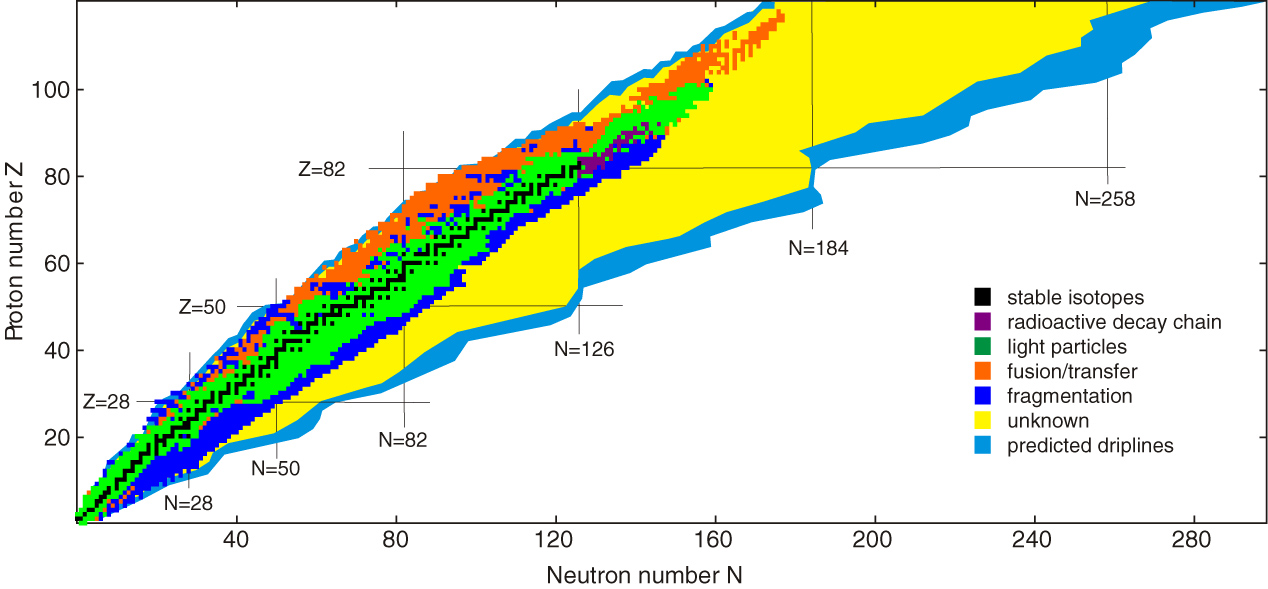
\includegraphics[width=.48\textwidth]{images/Intro_nuclearlandscape.jpg}
    \caption{The Segrè Chart visualising the nuclear landscape highlighting how the stability varies.\cite{famiano_nuclear_2019}.}\label{fig:intronuclan}
\end{figure}
    \section{The Theory of nuclear forces}
Ever since it was discovered that the nucleus is made up of protons and neutrons, scientists have been working out how it is held together.
The logical answer would be a force, though the only two forces known at the time were the gravitational and the electromagnetic.
However, neither of these could be the one as protons and neutrons don't have opposite charges and the gravitational force is far too weak to explain the phenomenon.
% So it was concluded it must be another force, called the nuclear force, which we now know to be residual effects of the strong force between quarks, another fundamental force.
So it was concluded it must be another force, called the nuclear force. \cite{hergert_guided_2020, machleidt_chiral_2011}

% citing [1], [2] for "residual", possibly textbooks, it's kinda basic stuff

\subsection{Exchange particles and meson theories}
The first theory for the nuclear force was developed by Yukawa, introducing his exchange particles.
From an intuitive standpoint, the Heisenberg uncertainty principle allows for short term spontaneous creation of particles \cite{machleidt_nuclear_2013}.
These particles can then transfer momentum between two nucleons, by interactions, before vanishing again.
This mechanism does impose certain range and strength constraints on the force however, as a stronger force requires more massive exchange particles, giving them less time to exist and travel between nucleons \cite{machleidt_nuclear_2013, hergert_guided_2020}.

Yukawa predicted the properties of suitable exchange particles and when the pion and other suitable mesons were discovered they gave rise to so called meson theories. % 1950s
Many properties of simpler interactions were explained well with One Boson Exchange (OBE) models, where only one exchange of each meson is considered \cite{machleidt_nuclear_2013}.
However, adapting the theory for multiple exchanges wasn't as straightforward and led to the development of many more advanced models (Paris, Bonn, Stony Brook) \cite{machleidt_nuclear_2013, machleidt_meson_1989}.

\subsection{Quantum Chromodynamics}
Then Quantum Chromodynamics (QCD) was developed, quarks were discovered, and the strong force was introduced between them, mediated by gluons.
This completely changed the picture of the nuclear force, as the attraction of nucleons was now attributed to residuals of the strong force, delegating the meson theories to models.
However, calculating the nuclear force directly from QCD is very difficult for a variety of reasons. QCD is highly nonperturbative at this range/scale, making it difficult to calculate, and even a two nucleon interaction would already involve six quarks.
Still, attempts are made using finite step computer simulations, called Lattice QCD, which are very useful for verifying simple interactions but aren't suitable for regular day-to-day applications \cite{machleidt_nuclear_2013,hergert_guided_2020}.

\subsection{Effective Field Theory}
Applying Effective Field Theory (EFT) was the next breakthrough, the key is that the significant effects may be studied independently at different scales.
To use EFT, one must first identify the degrees of freedom (the interacting particles/entities), in our case, nucleons and mesons (at the nucleon scale, mesons are the relevant exchange particles).
Then one constructs a Lagrangian (which is essentially an expression describing the dynamics of the system) in a certain way.
The key is to construct the most general possible Lagrangian that follows the same symmetries as the QCD strong force, as an expansion of $Q/\Lambda$.
Where $Q$ is the typical momentum of the system and $\Lambda$ the range at which the EFT interaction model stops being applicable.
The EFT application to QCD for modelling the nucleon interactions is called Chiral EFT (CEFT) as chirality (symmetry under reflection) is a key symmetry of the strong force \cite{machleidt_chiral_2011, machleidt_nuclear_2013, burgess_introduction_2007, hergert_guided_2020}.

Using CEFT is a rather involved process but the following tries to provide a short outline of the key features.
There are 2 main decisions, the first being how many nucleons do we include, the simplest being 2 nucleons (NN), following with 3 nucleons (3N), 4 nucleons (4N) and many nucleons.
The second is how many terms of the mentioned expansion do we take into account, these simplest here is regarded as the Leading Order (LO) followed by Next Leading Order (NLO), Next Next Leading Order (NNLO) and so on.
Determining both of these specifies which interactions need to be considered, \cref{fig:diagram1} shows Feynman diagrams for some.
In these there are different types of nodes each associated with a Low Energy Constant (LEC) which are determined by fitting experimental data and influence how the interaction affects the force \cite{machleidt_chiral_2011, machleidt_nuclear_2013, burgess_introduction_2007, hergert_guided_2020}.

\begin{figure}[H]
    \centering
    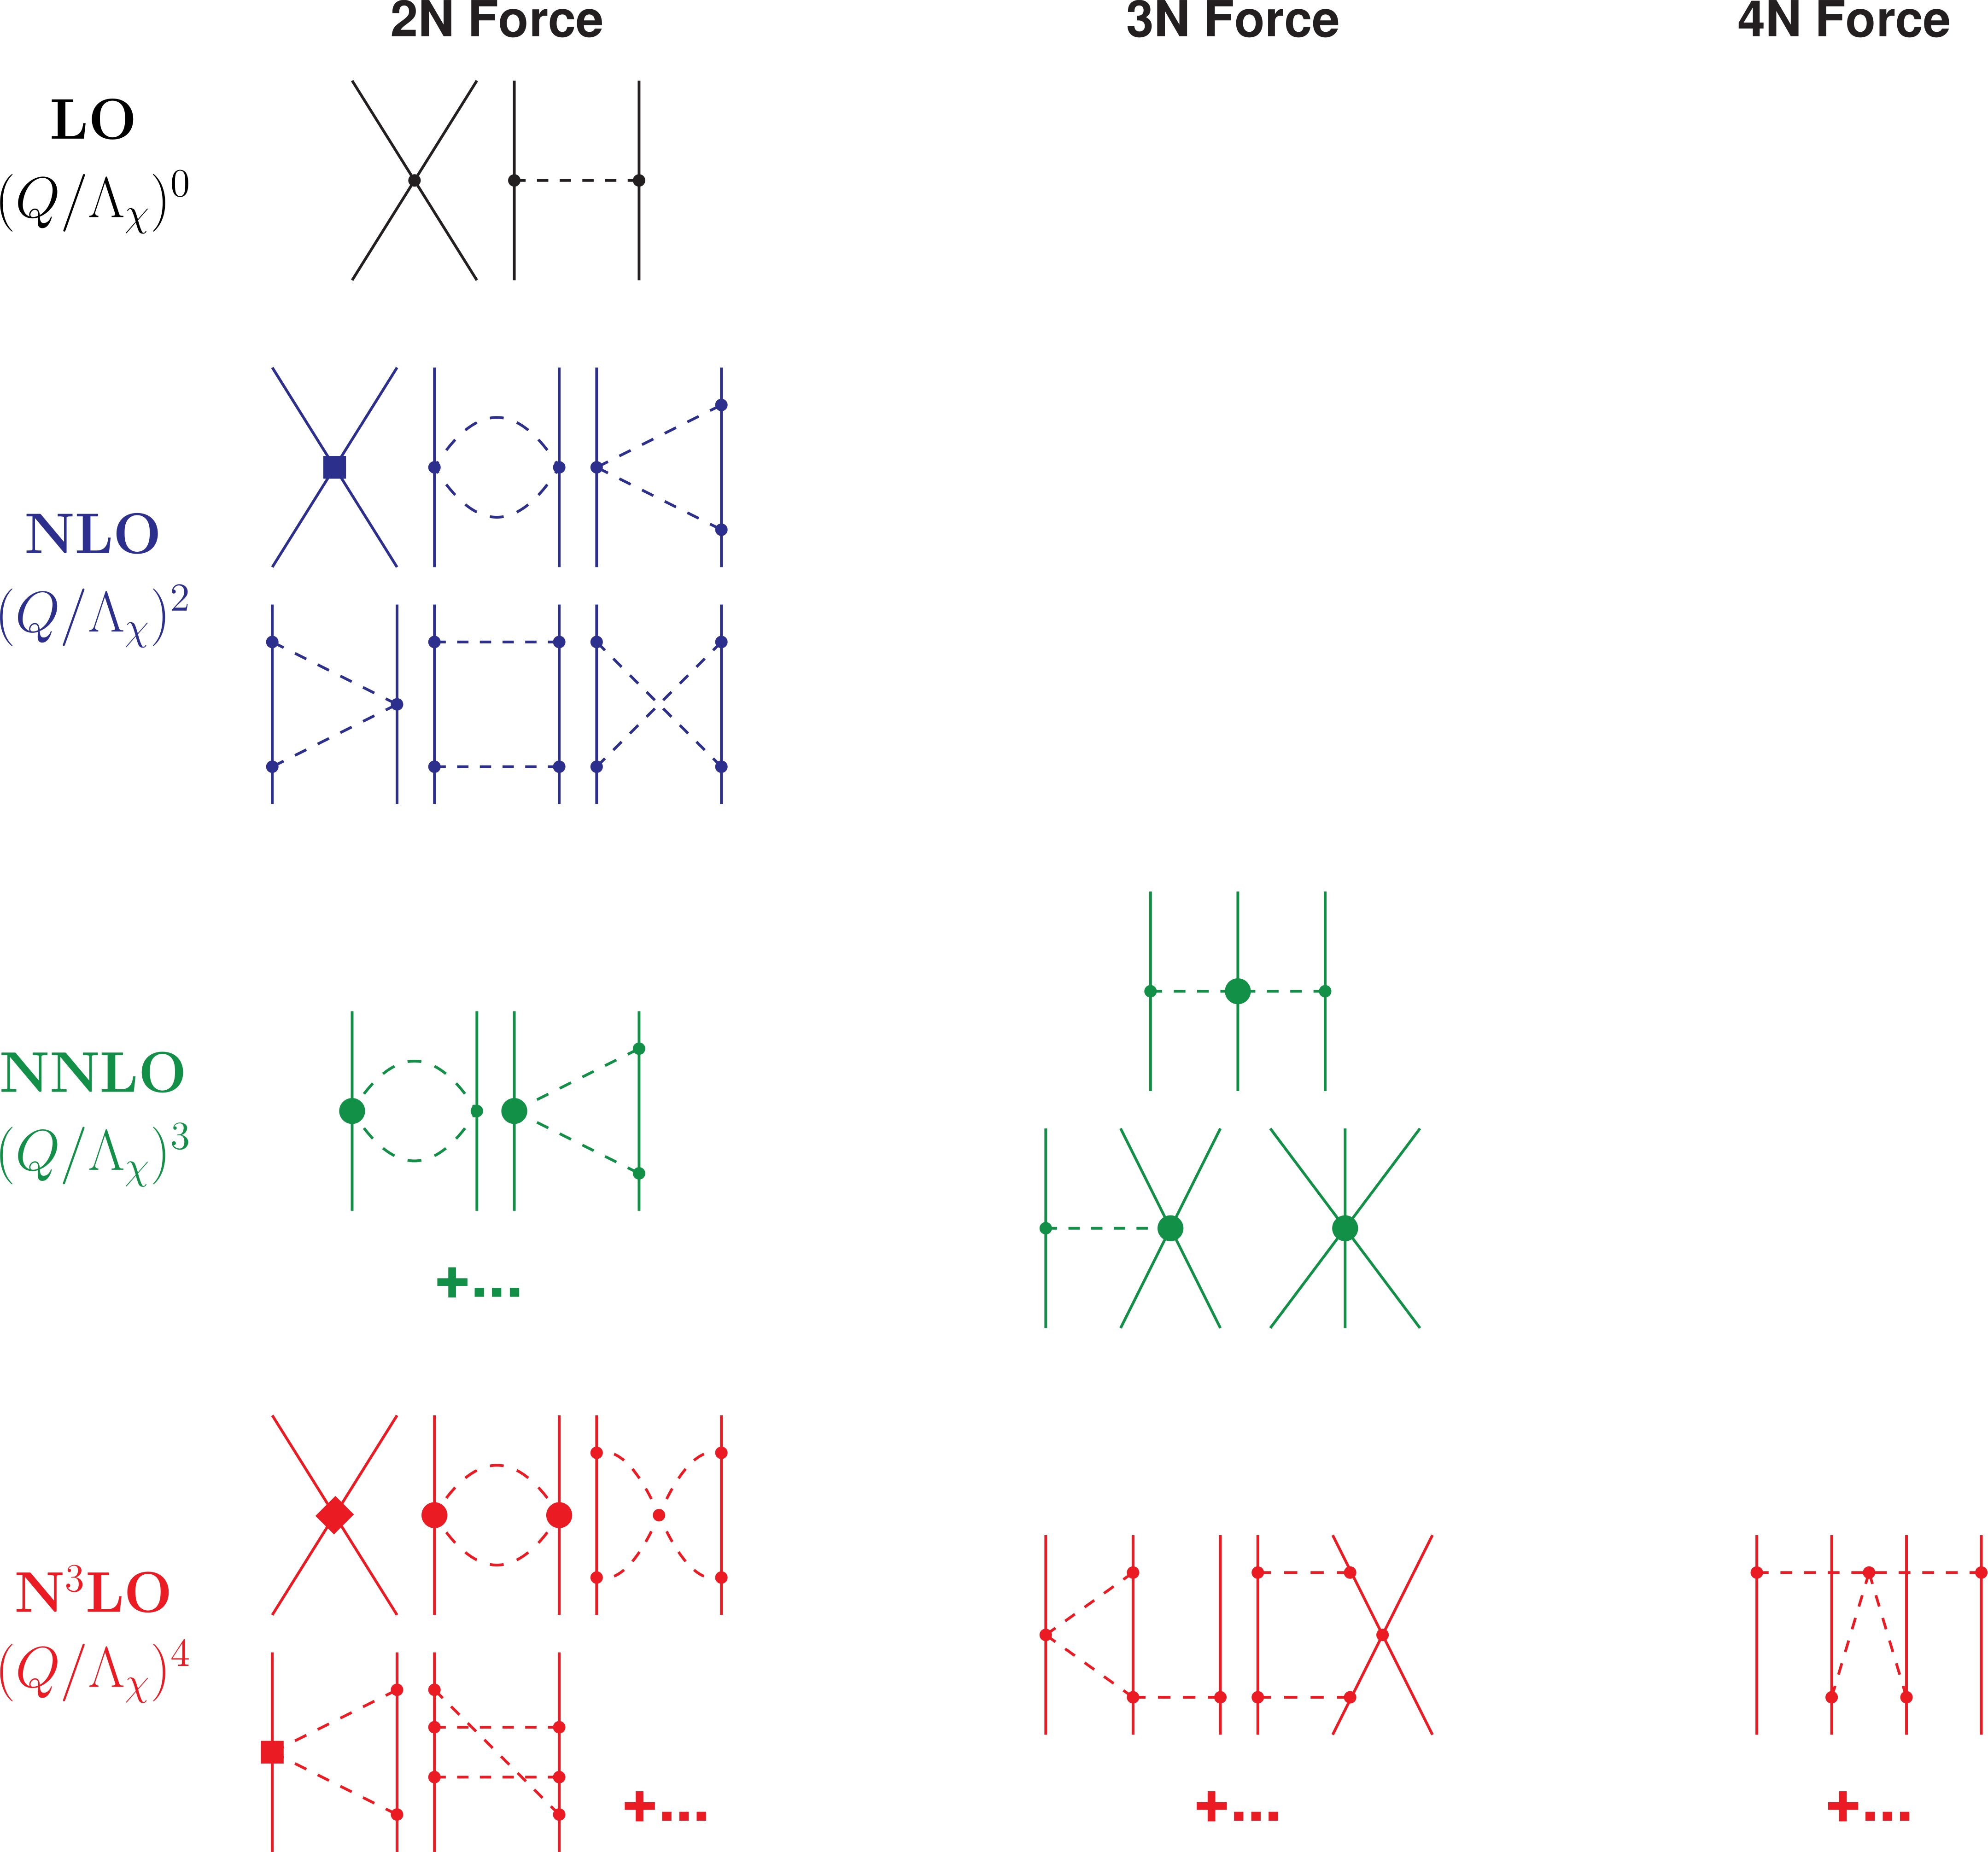
\includegraphics[width=.4\textwidth]{images/NFT_diagram.png}
    \caption{Feynman diagrams showing some of the first interactions that need to be considered when using CEFT. Solid lines represent nucleons and dashed lines pions. Different nodes represent different interactions \cite{machleidt_chiral_2011}.}\label{fig:diagram1}
\end{figure}

\subsection{Nuclear Shell Theory}
The nuclear shell model originates from scientists observing that atoms with certain numbers of protons and neutrons (called magic numbers, covered more later) were more stable than others, which resembled the effects of shell closures in the atomic shell model.
Simplest shell models consider the individual nucleons to behave independently, each in a potential formed by the many NN interactions, where this potential results in a central potential with additional spin-orbit, spin-spin and tensor components \cite{kruecken_introduction_2011}.


% The Nuclear Shell Model concerns the nuclear force from a different perspective, it is based on experimental observations made around the 1940s.
% Scientists have observed that atoms that have certain numbers of protons or neutrons are more stable (called the magic numbers and covered more in the following sections).
% These were taken as evidence for shell closures similar to those in the shell model of the atom, thus nuclear shell theory started.
% The underlying idea is that the nucleons within the nucleus move almost independently of each other, 

\subsection{Exotic nuclei}
From a practical point of view, most stable nuclei (especially ones in the valley of stability) are modeled well using combinations of the meson theories, CEFT based nuclear shell models (NN is often sufficient for stable isotopes) and other approaches.
However for exotic, neutron-rich nuclei the models fall short, at least 3N interactions need to be considered \cite{wienholtz_masses_2013} for an accurate model and more measurements are currently being made.
% However, most of the models fall short in some way, some need to be localized to be accurate enough, some are too computationally expensive to carry out for heavy isotopes and so on.
% After it was determined that for 
% Currently much work is being done on expending the CEFT approaches to contain more complicated nucleon

% Applying Effective Field Theory (EFT) was the next break through, EFT is somewhat similar to multipole expansion of electromagnetism. % cite the presentation
% The key is that the significant effects may be studied independently at different scales, to use EFT one must first identify the degrees if freedom (the interacting particles/entities), in our case nucleons and mesons.

% Applying Effective Field Theory (EFT) was the next break through, EFT is somewhat similar to multipole expansion of electromagnetism. % cite the presentation
% The key is that the effects of the strong force at the nucleon scale may be modeled without full understanding of all the details.
% EFT is a quantum theory and 

% cite [10]

% Applying Effective Field Theory (EFT) was the next break through, it allows approximating the QCD effects on a nucleon level.



    \section{Mass Spectrometry}
A Mass Spectrometer (MS) is a device used to measure the mass to charge ratio ($\frac{m}{Q}$) of ions.
Usually, this charge to mass ratio is calculated from either how much an ion is deflected in a magnetic field or accelerated in an electric field – ions with the same ratio are deflected/accelerated equally.
This information can be used for a variety of purposes such as determining an unknown isotope in a mixture or to directly measure nuclear masses.

The charge to mass ratio was first measured by J. J. Thomson in the late 19th century \cite{noauthor_j_nodate} and throughout the 20th century MS have evolved with numerous variations and different set ups.
This report focuses on 2 types of MS: the Penning trap and the Multiple Reflection Time of Flight (MR-TOF) mass spectrometer, as both are currently used to measure the mass of exotic nuclei \cite{famiano_nuclear_2019}.

\subsection{Importance to nuclear theory}
Mass spectrometers are integral to the study of nuclear theory for identifying or quantifying unknown samples (ions) as well as measuring binding energy of particles to gain information about their nuclear structure.
Nuclear mass is a fundamental property which has been responsible for the discovery of many nuclear effects such as shell closures and nucleon-nucleon pairing \cite{blaum_precision_2012}.
MS are used in nuclear physics research to explore exotic nuclei such as neutron rich calcium isotopes \cite{wienholtz_masses_2013} which are interesting to study as they can develop our understanding of the nuclear force.
Examining binding energy is key to understanding the nuclear theory, it is related to the stability of the nuclei so the atoms in the valley of stability have the lowest binding energy as well.
% Examining this excess mass “defect” is the most important metaphor of nuclear physics: “the valley of stability” which has the lowest mass excess.
% Overweight nuclides that farther away from equilibrium tend to have their mass excess with much shorter half-lives which is defined by the binding energy.

\subsection{How do mass spectrometers work}
% A general MS has three stages: an ioniser, mass analyser and a detector.
Firstly, a sample must be ionised before entering the mass analyser so it will interact with the magnetic and/or electric fields.
Ionization methods including thermal ionization, where the sample is heated and emits ions on its own, and electron impact, where the sample is bombarded by electrons to excite the sample atoms which then emit ions.
% In the mass analyser the beam is accelerated/deflected before being incident on a detector.
% The detector then measures the mass charge ratio based on the time or location of incidence \cite{noauthor_mass_nodate}.
Then the ions go through different processes depending on the type of MS and at the end, the ions are usually detected using an electron multiplier giving the number ions arriving at a given time \cite{noauthor_mass_nodate}.
% The more ions hit a certain part of the detector it means the sample has more of that type of isotope in nature.
% And from all that, MS can generate the spectrum which is useful for analysing unknown samples.

\subsection{Penning traps}
Penning traps are the most common MS in nuclear study where there are currently at least 7 active laboratories including CPT, ISOLTRAP, TITAN and SHIPTRAP, they give us the most precise measurements for stable isotopes \cite{huang_ame_2021}.
Just 15 years ago, the only Penning trap spectrometer publishing the masses of radioactive samples was the pioneering experiment ISOLTRAP, set up at CERN’s ISOLDE facility in 1986 \cite{lunney_new_2019}. % RRR
Penning traps are based on a cyclotron design, and they trap the isotopes using a combination of strong longitudinal uniform magnetic and an quadrupole electric fields, high homogeneity also reduces the possibility of field drifts so that they move periodically and the frequency is related to mass following the equation
\begin{equation}
    \nu_c = \frac{1}{2\pi}\frac{qB}{m}
\end{equation}

To perform a mass measurement we then trap our sample in a Penning trap and scan through the suspected frequencies and measure the resonant response.
The response will be highest when many ions orbit at the given frequency, usually the sample would include an ion the mass of which is to be measured and a reference ion of known mass, the frequencies and masses are then related to each other.
From this also stems the main feature of Penning traps, it takes time to scan through the frequencies, meaning the more time available the more precise the measurement \cite{konig_quadrupole_1995}.

% The measured quantity is cyclotron frequency which can be essentially measured in high accuracy.
% Also, the coexistence of trapping and cooling minimizes systematic errors from mass measurement though the time it takes to complete a cycle is the main limitation of mass measurement which tends to limit the range of isotopic species that can be measured \cite{famiano_nuclear_2019}.

\begin{figure}[H]
    \centering
    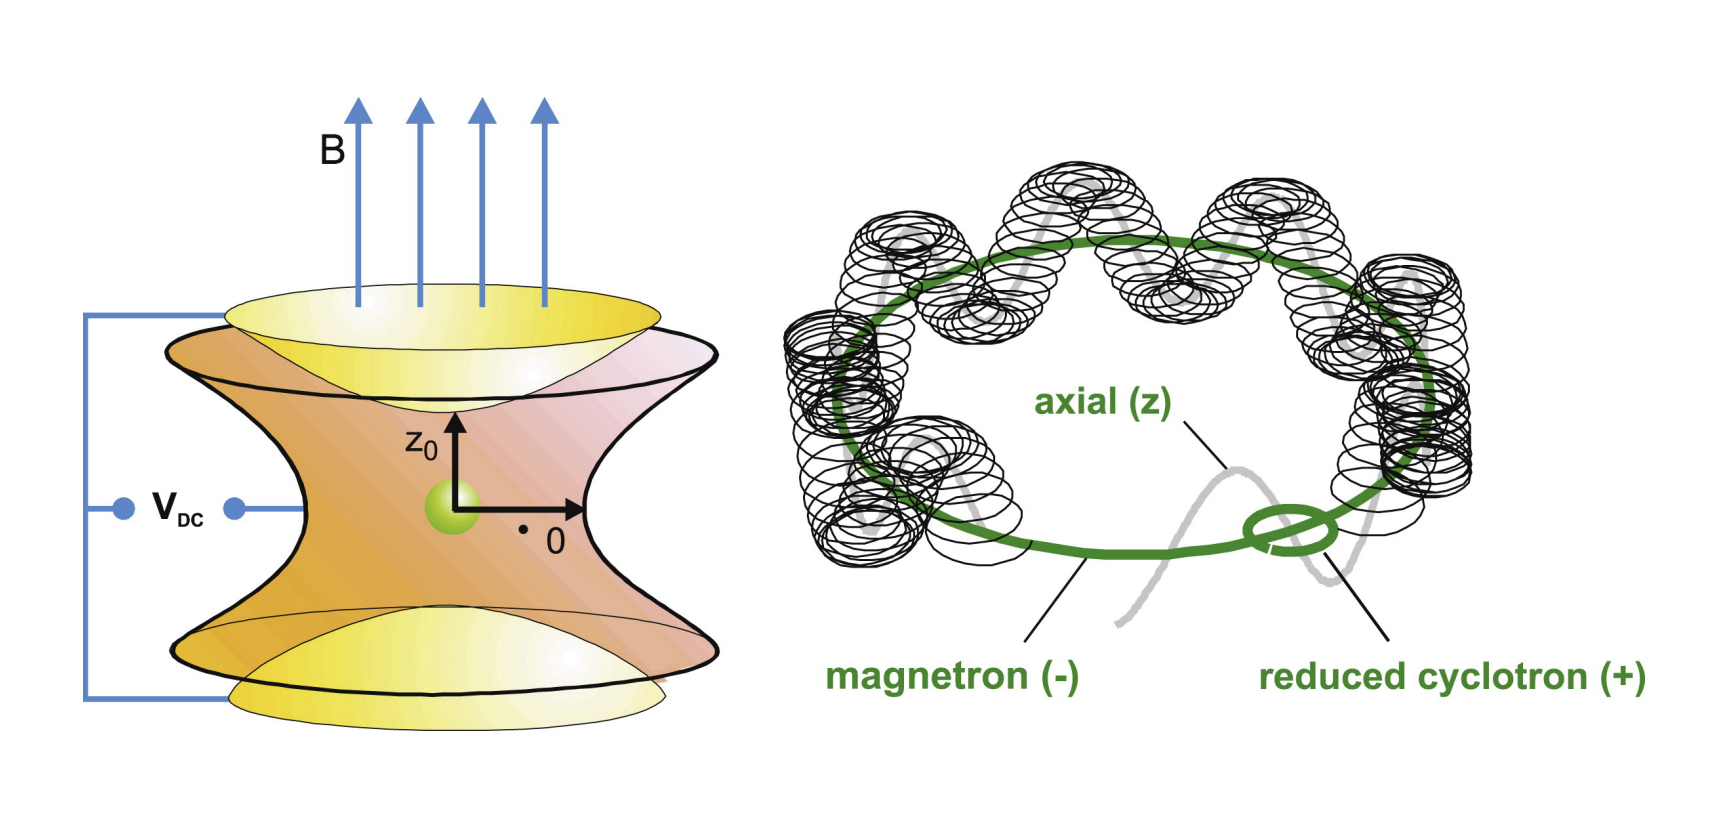
\includegraphics[width=.5\textwidth]{images/MS_penningtrap.png}
    \caption{Schematic diagram of a Penning trap \cite{famiano_nuclear_2019}.}\label{fig:MS_PT}
\end{figure}

\subsection{MR-TOF mass spectrometers}
MR-TOF devices are the newest ion-trap development, first being used in 2013, they are often used accompanied with Penning traps.
Their greatest advantage is that they can provide measurements for isotopes with very low production rates and very short half-lives, which is particularly suitable for short lived nuclei as they can resolve in less than 30ms and are suited to rare nuclei as they can resolve small sample sizes \cite{wolf_isoltraps_2013}.
MR-TOF MSs work by reflecting the ions back and forth between two electrostatic mirrors in a short tube, effectively increasing the flight path length.
The key is that the speed of the ions depends on the mass-to-charge ratio, so after a while, the isotopes are detected, and the mass is calculated from the time of arrival through this equation
\begin{equation}
    t = \frac{d}{\sqrt{2U}}\sqrt{\frac{m}{q}}
\end{equation}

The main benefit of MR-TOF compared to Penning traps is that there is no need to scan through a variable.
The atoms simply arrive at the time and very high mass resolving power can be achieved in a small time, making them very well suited for measurements of very unstable nuclei (neutron rich in particular).
This is visualised in \cref{fig:MSPTMRTOF} which shows the achievable mass resolving power given an available observation time of a Penning trap and MR-TOF present at ISOLTRAP in CERN.

% MR-TOF MSs are usually faster and more sensitive as a non-scanning device with high ultra-mass resolving power than a Penning trap.
% It has several advantages compared to a frequency-based mass spectrometer also including the single-ion sensitivity, short cycle time (5ms) and superior resolving power for a measurement time of 1s and mass-to-charge ratio larger than hundreds of amu \cite{dickel_multiple-reflection_2013}.

\begin{figure}[H]
    \centering
    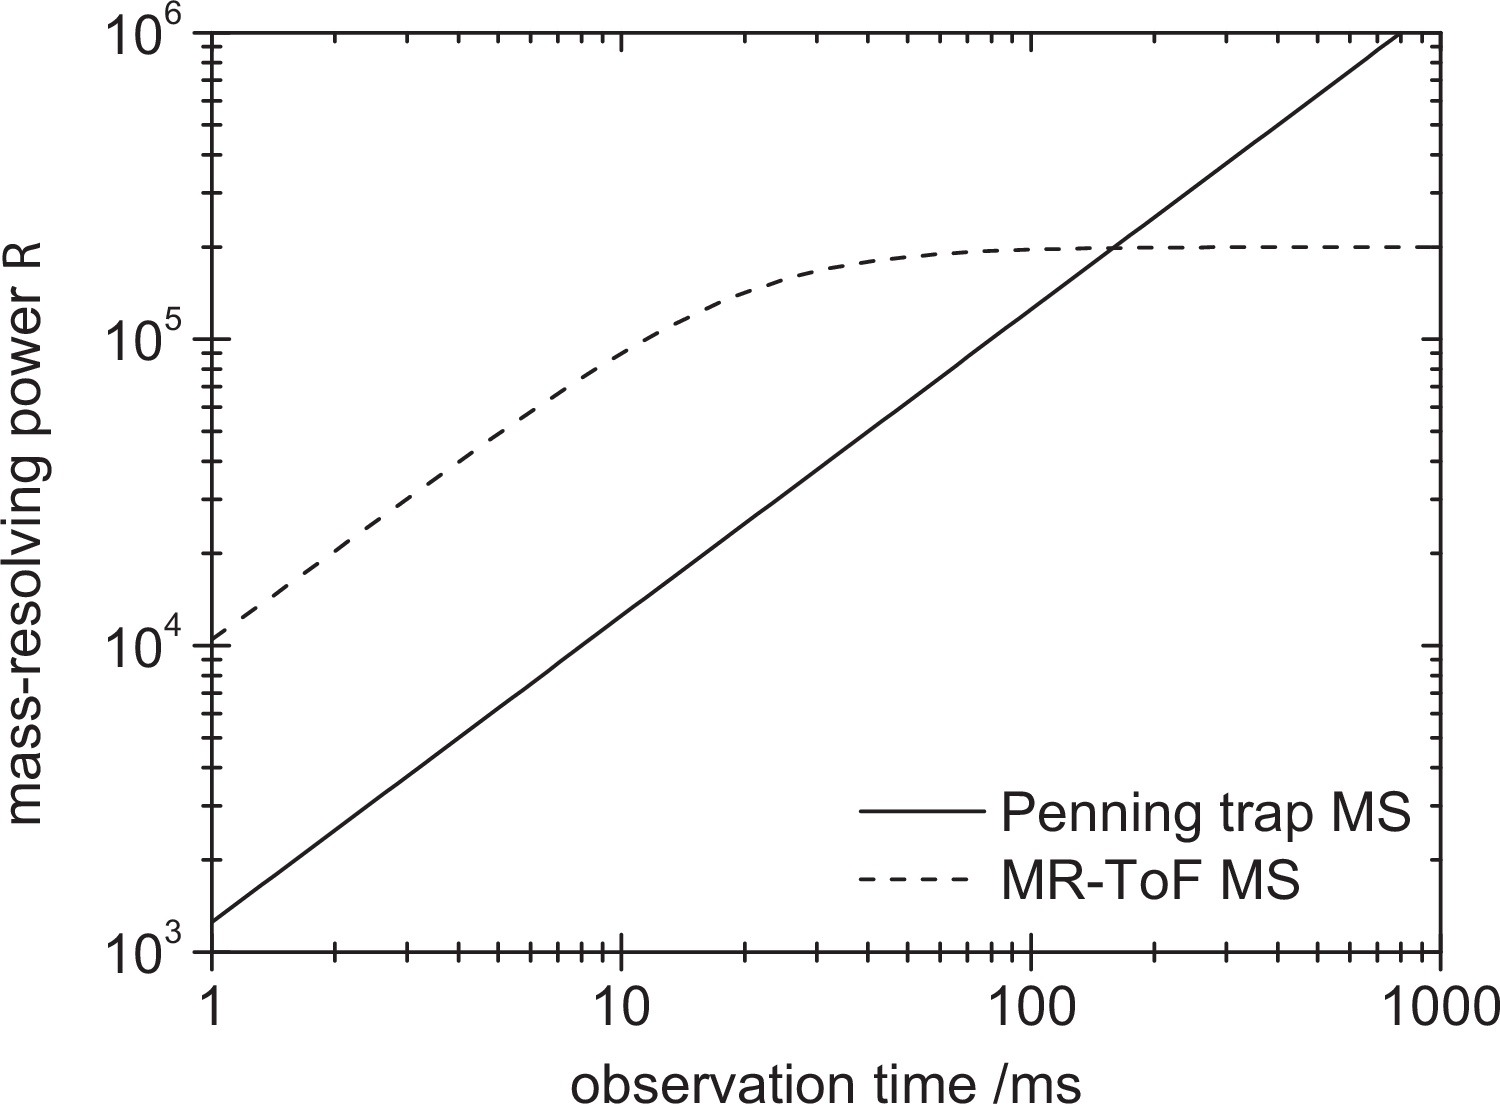
\includegraphics[width=.5\textwidth]{images/MS_PTMRTOF_graph.jpg}
    \caption{The mass resolving power as a function of observation time for a Penning trap and MR-TOF MS. The MS compared are both from the ISOLTRAP experiment at CERN.
    \cite{wolf_isoltraps_2013}}\label{fig:MSPTMRTOF}
\end{figure}

    \section{Nuclei mass measurements with regard to nuclear force theory}
The mention of binding energy and results was previously stated.
Another analysis we could do on nucleon binding energies is investigating the magic numbers of nucleons.
The idea is that there is a section on the nucleon landscape that is stable.
Before the discovery of the standard 2, 8, 30, 28, 50, 82, 126 magic numbers, higher values of 184, 258, 350, and 462 are thought to exist. 
The existence of these number are theoretical and are calculated based on the Binomial coefficient.

\subsection{Nucleon pairing energy}
Besides the standard investigations, we can also investigate the neutron pairing energy of finite nuclei.
We can study a range of odd and even pairs of N/Z numbers; to investigate the strong nuclear force \cite{fred_neutron_2019}.
So far, the idea is that the (N)even-(Z)even nucleus (although energy depends on factors such as the kind of particles and state it is occupied) we known for a fact that odd(N)- odd(A) nucleus is 1/2 to 2/3 times smaller, this is when they are given in the same shell and the mass numbers A are very close to one another.
This strange character is due to the nucleon-nucleon potential resulting from the strong force. \cite{jensen_elementary_1955}

There is a model known as the liquid drop model, which underpredicts the binding energy of magic nuclei, magic nuclei referrer to nuclei where N or Z are a magic number, for the stable atoms these are 2, 8, 20, 28, 50, 82 and 126.
The neutron/proton separation energy peaks if N(Z) equals a magic number; on \cref{fig:MSaNFTzigzag}, we see this as the last point before the significant drop.
There is a more stable isotope if Z is a magic number and a more stable isotone if N is a magic number.
If either N or Z or both are magic numbers, then the energies of the excited state will be much higher than the ground state.
Another discovery is that elements with Z equal to a magic number have a more prominent natural abundance than nearby elements. \cite{kumawat_description_2018}

\begin{figure}[H]
    \centering
    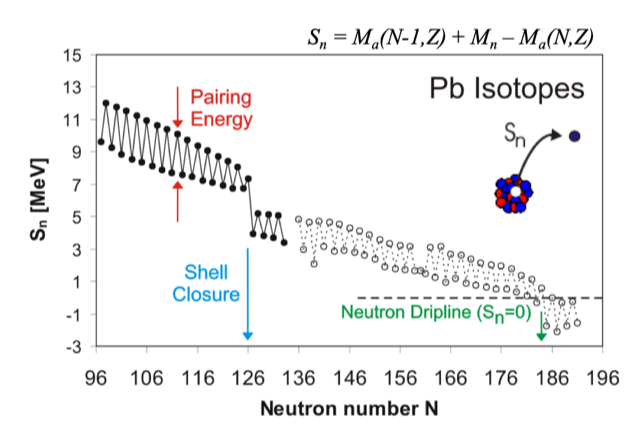
\includegraphics[width=.5\textwidth]{images/MSaNFT_zigzag.png}
    \caption{Neutron binding energy for lead isotopes. In blue a shell closure is highlighted at 126N. The sharp oscillations in energy highlight neutron pairing energies \cite{noauthor_nuclear_nodate}.}\label{fig:MSaNFTzigzag}
\end{figure}

\subsection{Liquid drop model and the investigation of magic numbers}
The magic number can further be explained by the shell closure model of the nucleus.
This is done by considering each nucleon to be moving in some potential and classifying the energy level in terms of quantum numbers n l j, like how the wavefunction of individual electrons are classified in atomic physics.
The energy eigenvalues depend on the principal quantum number, n, orbital angular momentum.
The energy level comes in shells, with a large gap just above each shell. \cite{smolanczuk_particle}

\subsection{Nucleon driplines}
In particle physics, we often use the idea of drip lines to categorize our particles.
We have a one or two-particle drip line, which is a result of the idea that odd and even nucleon numbers, as we know, it has a significant effect on binding energy.
We will be looking at one particle drip line for an odd(Z) or odd(N) nuclei.
Experimentally, we determined the one and two neutron drip lines up to neon. [??tobedone??]
    \section{Applications of MS outside nuclear force theory}

Mass spectrometry has a long history and wide adoption out with nuclear physics both in research and commercially.
MS are essential for chemical analysis – often used to determine the isotopes present in a mixture.
In chemical and biomedical research, they are used frequently for structural elucidation where MS can give information about molecular structure. \cite{bhattarai_chapter_2020}

\subsection{Penning traps and neutrino physics}
One exciting area of study where MS are fundamental is neutrino physics.
The neutrino is the most abundant particle with mass - roughly a thousand trillion pass through your body every second. \cite{noauthor_whats_nodate}
Yet the incredibly light particles are elusive and difficult to detect as they only interact with the weak force and gravity so surprisingly little is known about them. \cite{noauthor_what_nodate}
Research in neutrino science could further the understanding of the standard model and they could be important in explaining why there is matter in the universe and not antimatter \cite{gibney_morphing_2015} – it is thought that neutrinos could be their own antimatter, unlike any other fermion in the standard model [8]. 
Penning traps are especially suited to this study due to their high (precison/resolving power).
Since neutrinos are chargeless themselves, an upper limit to their rest mass can be measured by the mass difference between mother and daughter nucleotides from a nuclear decay. \cite{eliseev_penning-trap_2013}
For example the $\beta$ -decay: $^{187}Re \longrightarrow ^{187}Os + e^- + \bar{\nu _e}$ with Rhenium as the mother nucleotide and Osmium the daughter. \cite{repp_pentatrap_2012}
The current upper limit of this mass is 1.
1eV measured at the Karlsruhe Tritium Neutrino (KATRIN) spectrometer. \cite{castelvecchi_physicists_2019}
Although KATRIN is an electron spectrometer and not a MS, PENTATRAP is a new five Penning trap facility being built in Heidelberg, Germany and is expected to reduce this upper mass limit even further \cite{repp_pentatrap_2012}.

\subsection{MR-TOF's applications outside physics}
MR-TOF MS also have many applications outside nuclear physics.
Due to their compact size and relative affordability compared to Penning traps, MR-TOF's are suited to \emph{in situ} applications \cite{dickel_multiple-reflection_2013}.
One potential application is waste water management where the MS could identify pollutants \cite{dickel_multiple-reflection_2013} – during COVID-19 pandemic waste water analysis was used to model the spread of the disease \cite{noauthor_wastewater_nodate}.
One current application of the technology is in biomedical analysis where a variation of the device (MALDI-TOF MS) is used routinely as an accurate and fast method to identify of microorganisms which reduces costs as it requires minimum consumables. \cite{noauthor_uk_2019}
    \section{Summary}
Studies of the nuclear force are a fascinating yet unfinished part of physics.
Though most simple interactions involving it are well understood, it is yet to be applied to more complicated systems.
Mass spectrometers have been crucial in testing nuclear theories and pushing their limits.
They have allowed for the exploration of the nuclear landscape closer to the neutron dripline where models using only 2N interactions have been insufficient in predicting the shell closures of these exotic nuclei.
Future MS such as the PENTATRAP experiment \cite{repp_pentatrap_2012} or the many MR-TOF spectrometers that are being developed, with improved resolving power and shorter needed observation time will be crucial in probing and improving the leading nuclear force theories.

% In summary, the current research outlines the role of mass spectrometers in ongoing work in the field of nuclear physics.
% Nuclear physicists works on determining different masses of the nucleus and different isotopes and works on the fundamentals; we can build on a better future through this work.
% However, it is clear that there are still much to prove and disproof, and currently, we do not know how much is unknown.
% Nevertheless, there are many applications of mass spectrometers we are happy with; from water treatment to uses in space exploration, the technology of MS had a considerable impact on our lives.
    
    \printbibliography

\end{multicols}

\end{document}
